\documentclass[a4paper,12pt]{article}
\usepackage{graphicx}
\usepackage{hyperref}
\usepackage{amsmath}
\usepackage{times}
\usepackage{xcolor}
\usepackage{amsfonts}
\usepackage{garamondx}
\usepackage{framed}  %This is to use the shaded environment

\usepackage{titlesec}

\titlespacing*{\section}
{0pt}{5.5ex plus 1ex minus .2ex}{4.3ex plus .2ex}
\titlespacing*{\subsection}
{0pt}{5.5ex plus 1ex minus .2ex}{4.3ex plus .2ex}

\usepackage{titling}
\setlength{\droptitle}{-8em} 


\textwidth=6.2in
\textheight=8.5in
%\parskip=.3cm
\oddsidemargin=.1in
\evensidemargin=.1in
\headheight=-.3in
\setlength{\parindent}{0pt}



% \renewcommand{\baselinestretch}{1} 
% \setlength{\parskip}{\baselineskip}
% \setlength{\parindent}{0pt}
% \setlength{\marginparwidth}{2.5cm}


\newcommand{\scscst}{\scriptscriptstyle}
\newcommand{\scst}{\scriptstyle}
\newcommand{\Robject}[1]{{\code{#1}}}
\newcommand{\Rfunction}[1]{{\code{#1}}}
\newcommand{\Rclass}[1]{\textit{#1}}
\newcommand{\Rpackage}[1]{\textit{#1}}
\newcommand{\Rexpression}[1]{\code{#1}}
\newcommand{\Rmethod}[1]{{\code{#1}}}
\newcommand{\Rfunarg}[1]{{\code{#1}}}

\newcommand\boldblue[1]{\textcolor{blue}{\textbf{#1}}}
\newcommand\code[1]{\textcolor{red}{\texttt{#1}}}

\usepackage{Sweave}
\begin{document}
\Sconcordance{concordance:3_Course_Notes-knitr.tex:3_Course_Notes-knitr.Rnw:%
1 50 1 1 0 4 1 1 7 12 1 1 7 1 1 1 7 94 1 1 2 1 0 3 1 3 0 1 2 6 1 1 2 1 %
0 1 1 1 2 1 1 3 0 1 2 9 1 1 2 4 0 1 2 4 1 1 2 1 0 1 1 3 0 1 2 45 1 1 4 %
6 0 1 2 12 1 1 2 4 0 1 2 5 1}

\definecolor{shadecolor}{gray}{0.95} %this is defining the color of the background in the shaded environment

%\SweaveOpts{concordance=TRUE}



%------------------------------------------------------------
\title{Using R as a Research Tool.}
%------------------------------------------------------------
\author{Susan Johnston: \href{mailto:Susan.Johnston@ed.ac.uk}{Susan.Johnston@ed.ac.uk}  \\ \\
        Demonstrators: Gergana Dalaskova, John Godlee. \\
        Hat-Tips to Kyle Dexter, The Coding Club and R4all.}
%\date{}









\maketitle

%\tableofcontents


%-------------------------------------------
\section {Introduction}
%--------------------------------------------

\subsection {What is \boldblue{R}?}

\boldblue{R} began its life in New Zealand in 1993 as a language and environment for statistical computing and graphics. It is an interpreted programming language, meaning that rather than pointing and clicking, the user types in commands. It is \textbf{free} and works across all platforms.


\subsection {Why use \boldblue{R}?}

\begin{center}
``\texttt{This is R. There is no if. Only how.}'' \\
\texttt{{-}{-} Simon `Yoda' Blomberg, R-help (April 2005)}

\end{center}


Almost anything is possible in \boldblue{R}. It is fast becoming the \textit{lingua franca} of academic research and data science. It is used for:

\begin{itemize}
\item Processing and tidying data 
\item Statistical analyses
\item Data visualistion (\texttt{ggplot})
\item Creating interactive web applications (\texttt{shiny})
\item Generating reports and presentations (\texttt{knitr}, \texttt{slidify})
\item Creating portable projects (RStudio Projects)
\end{itemize}

The analytical power of \boldblue{R} lies in its many packages (11,172 at the time of writing). At least 300 of these are written for ecologists and evolutionary biologists. A list of packages are hosted on the Comprehensive R Archive Network (known as \textbf{CRAN}): \url{https://cran.r-project.org/}.

% \subsection {What we hope to achieve in this session.}
% 
% Before beginning this course, we asked you to complete the 


%-------------------------------------------
\section {Getting Started: R and the RStudio Environment.}
%--------------------------------------------
\subsection {Installing R and RStudio.}

R can be downloaded from the CRAN website. Whilst the CRAN download version provides a simple user interface, we recommend that R is run through the software RStudio. This is open-source, free, and available at \url{http://www.rstudio.com/}. [NB. It is important to install R first and RStudio second.]


\subsection {Creating an R Project.}

Using R Projects (\texttt{.RProj}) is not necessary, but we strongly recommend that you use them. The advantage using R Projects is that it allows easier file imports, improved reproducibility and collaboration. This is primarily because it tells R where to look for data files and scripts, meaning that a script can be run on machine to another without any problems. \\

We have provided you with the project \texttt{Intro\_to\_R.RProj}. Opening this file will open RStudio. On the Files tab in the lower right corner, you will see the files in the current working directory. This will be useful later when we tell R to load files. You can check the working directory by typing \code{getwd()}. \\

If you would rather not use projects, you can set the working directory by using the command \code{setwd()} or by selecting \texttt{Session > Set working directory > Choose directory}. \\

Creating an R Project is straightforward: select \texttt{File > New Project} and follow the instructions.


\subsection {Using RStudio.}

Open \texttt{Intro\_to\_R.RProj} and open the example R Script (\texttt{File > Open File... > 1\_Example\_Script}). RStudio should look something like Figure \ref{fig:R_Studio}. 
\\


\begin{figure}[h]
	\centering 
	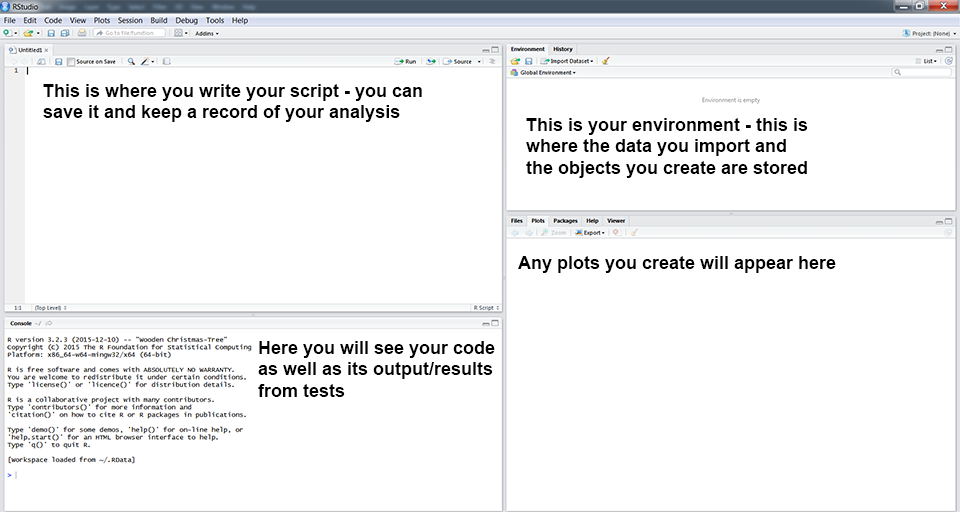
\includegraphics[width=1.1\textwidth]{figs/R_Studio.png}
	\caption{The RStudio Environment. Taken from OurCodingClub.io}
	\label{fig:R_Studio}
\end{figure} 

On the lower left is the \textit{Console} pane - this is the engine of R. You can give instructions to R by directly typing at the prompt (\code{>}). 
\\

On the upper left is your R Script - here, you can write commands and send them to the console by clicking ``\texttt{Run}'' or by typing \code{Ctrl-Enter} (or \code{Cmd-Enter}). Notice that all lines are preceded by \code{\#} - this is the comment character in R.
\\

On the lower right, you can browse the packages installed on your machine, open files and search R Help. This pane will also show plots when we run them later in the practical.
\\


\fbox{\begin{minipage}{36em}
\Large{\textbf{Exercise 1.}}

\normalsize
Try running some basic commands directly in the console and from the R Script:
\end{minipage}}


\begin{shaded}
\begin{Schunk}
\begin{Sinput}
> 2+3
> 1:10
> seq(1, 20, 4)
> mean(c(3, 6, 9, 3, 6, 7))
\end{Sinput}
\end{Schunk}
\end{shaded}

\fbox{\begin{minipage}{36em}
Let's assign a sequence of numbers to an object, \code{x}:
\end{minipage}}

\begin{shaded}
\begin{Schunk}
\begin{Sinput}
> x <- 1:10
> x
> y <- seq(0, 4.5, 0.5)
> y
\end{Sinput}
\end{Schunk}
\end{shaded}


You can see that in the upper right pane, we can see this new objects \code{x} and \code{y} in the environment.

\subsection {Finding Help within R.}

The fastest way to find help in R is to search using \code{?}. For example:

\begin{shaded}
\begin{Schunk}
\begin{Sinput}
> ?mean
\end{Sinput}
\end{Schunk}
\end{shaded}

should bring up a help page for the function \code{mean()} in the lower right corner. Typing two question marks: 

\begin{shaded}
\begin{Schunk}
\begin{Sinput}
> ??mean
> ??"standard error"
\end{Sinput}
\end{Schunk}
\end{shaded}

will search all help files and return a list of those that match. \\\\

\fbox{\begin{minipage}{36em}
\Large{\textbf{Exercise 2.}}

\normalsize
\begin{enumerate}
\item Using only \code{?} and/or \code{??}, find a function for calculating the standard deviation. What is the standard deviation of \code{x}?

\item Using \code{?}, find the help file for the \code{sort()} function. Sort \code{x} and \code{y} in reverse order.\\
\end{enumerate}
\end{minipage}}


\subsection {Troubleshooting and finding help outside of R.}

\begin{itemize}
\item Coding Club Tutorials \& Useful Links \url{https://ourcodingclub.github.io/}
\item Stack Overflow \url{https://stackoverflow.com/}: Try searching with the tag [R]
\item RStudio Cheatsheets \url{https://www.rstudio.com/resources/cheatsheets/}
\end{itemize}


%-------------------------------------------
\section{Loading data into R.}
%--------------------------------------------

Now that we are familiar with the RStusio environment, it's time to start working with real data. \\

In the folder \texttt{data}, you have been provided with a single dataset on Peruvian Soil in two common formats - \texttt{.txt} (tab-delimited) and \texttt{.csv} (comma-delimited). \\

The easiest way to read the data into R is to use the \texttt{Import dataset} button in the Environment tab, selecting \texttt{From Text (base)...} and choosing either datafile (\texttt{.txt} or \texttt{.csv}). A box will appear (Figure \ref{fig:Import_Dataset2}). Check each of the options that applies to the data (i.e. change nothing) and click ``\texttt{Import}''. You will notice that the object \texttt{Peru\_Soil\_Data} is now in the R environment, but you may also have noticed a command appearing in the Console: \\


\begin{figure}[t]
	\centering 
	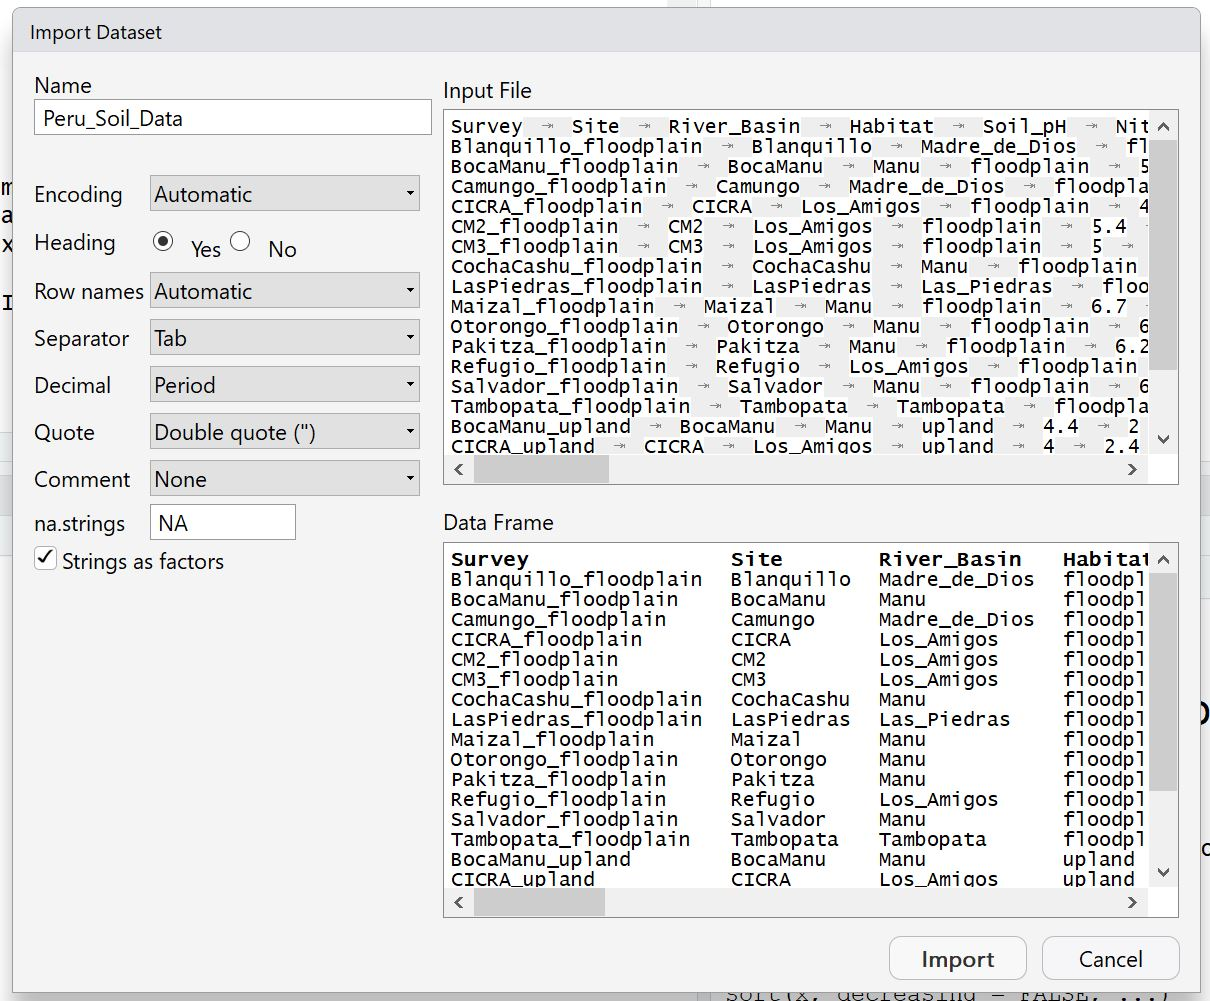
\includegraphics[width=0.8\textwidth]{figs/Import_Dataset2.JPG}
	\caption{Importing data manually into R}
	\label{fig:Import_Dataset2}
\end{figure} 



\begin{shaded}
\begin{Schunk}
\begin{Sinput}
> Peru_Soil_Data <- read.delim("C:/Users/sjohns10/Google Drive/
+ Teaching and Seminars/201711 NERC E3 DTP/Intro_to_R/data/
+ Peru_Soil_Data.txt")
\end{Sinput}
\end{Schunk}
\end{shaded}

This command can be copied and pasted into your script, which would save you from clicking the next time. However, providing such a long path if problematic - if you were to rename one of the directories, or move the folder somewhere else, then the code would no longer work. \\

RProjects provide the solution to this. Try typing the following into your script, and guiding the command to the data file using the \texttt{Tab} key:

\begin{shaded}
\texttt{Peru\_Soil\_Data <- read.delim("}
\end{shaded}

You should now have the following code in your script:

\begin{shaded}
\begin{Schunk}
\begin{Sinput}
> Peru_Soil_Data <- read.delim("data/Peru_Soil_Data.txt")
\end{Sinput}
\end{Schunk}
\end{shaded}


We recommend that instead of \code{read.delim()}, that you use either \code{read.table()} or \code{read.csv()}, as they offer more flexibility on defining various features about the input files. \\\\


\fbox{\begin{minipage}{36em}
\Large{\textbf{Exercise 3.}}
\\

\normalsize
Using \code{?}, find the help page for \code{read.table}. Read the file \texttt{Peru\_Soil\_Data.txt} into R. Check the loaded object using the \code{head()} function. Do you need additional arguments to read in the file properly?

\end{minipage}}\\

{ }
The object \texttt{Peru\_Soil\_Data} is a type of object known as a data frame. You can explore the data visually by clicking on its entry in the Environment tab. Alternatively, there are functions in base R that are good for telling you what your data look like. For data frames, these include \code{head()} and \code{str()}. Try these out.


%-------------------------------------------
\section{Data management in R.}
%--------------------------------------------

Exploring and manipulating data is fundamental to data analysis. In this section, we will briefly cover how to sort and filter the soil dataset. There are several approaches to doing this in the base code of R, but here we will use on the functions \code{select()}, \code{filter()} and \code{arrange()} from the package \textbf{\texttt{dplyr}}. \\

First, we need to load the \texttt{dplyr} package. It is good practise to do this at the beginning of the script when you are setting up the working environment.

\begin{shaded}
\begin{Schunk}
\begin{Sinput}
> library(dplyr)
\end{Sinput}
\end{Schunk}
\end{shaded}

\fbox{\begin{minipage}{36em}
NB. Some of you may get an error message:\\
\code{Error in library(dplyr) : there is no package called `dplyr'} \\

In this case, the library has to be installed from CRAN. This can be done by typing \code{install.packages("dplyr")}. It may ask you to select a mirror - select the RStudio Global mirror, or one that which is geographically closest to you. \\

\end{minipage}}

\subsection{Summary Statistics.}

Functions such as \code{head()} and \code{str()} are useful to telling you what your data look like, but don't give much information on what the data say.\\

A versatile function for exploring objects is \code{summary()}. This function summarises each numeric column in terms of the median, mean, interquartile range, minimum and maximum. It also provides information on levels and sample sizes for categorical variables. 

\begin{shaded}
\begin{Schunk}
\begin{Sinput}
> summary(Peru_Soil_Data)
\end{Sinput}
\begin{Soutput}
         Site           River_Basin       Habitat      Soil_pH     
 BocaManu  : 2   Las_Piedras  : 2   floodplain:14   Min.   :4.000  
 CICRA     : 2   Los_Amigos   : 8   upland    :11   1st Qu.:4.500  
 CM2       : 2   Madre_de_Dios: 2                   Median :5.200  
 CM3       : 2   Manu         :11                   Mean   :5.228  
 CochaCashu: 2   Tambopata    : 2                   3rd Qu.:5.900  
 LasPiedras: 2                                      Max.   :6.700  
 (Other)   :13                                                     
 Nitrate_Nitrogen   Phosphorus       Calcium         Magnesium    
 Min.   :0.00     Min.   : 1.80   Min.   :  39.0   Min.   : 10.5  
 1st Qu.:0.50     1st Qu.: 3.50   1st Qu.: 104.5   1st Qu.: 22.0  
 Median :1.40     Median : 4.30   Median : 543.0   Median :125.5  
 Mean   :1.26     Mean   : 9.44   Mean   : 875.6   Mean   :127.7  
 3rd Qu.:2.00     3rd Qu.: 6.50   3rd Qu.:1853.0   3rd Qu.:226.0  
 Max.   :2.40     Max.   :57.00   Max.   :2292.0   Max.   :323.0  
                                                                  
   Potassium        Sodium         Manganese    
 Min.   :14.5   Min.   :  3.50   Min.   :  5.0  
 1st Qu.:27.0   1st Qu.:  5.00   1st Qu.: 15.0  
 Median :35.5   Median :  7.50   Median : 24.5  
 Mean   :42.7   Mean   : 13.05   Mean   : 33.9  
 3rd Qu.:63.1   3rd Qu.: 11.00   3rd Qu.: 44.1  
 Max.   :88.5   Max.   :136.00   Max.   :103.5  
\end{Soutput}
\end{Schunk}
\end{shaded}

\subsection{Sorting data with \code{arrange()}}

There are occasions where it is useful to have sorted data, either because we would like to examine it, or for some types of statistical analyses i.e. with time-series data. The \code{arrange()} function sorts data frames as so:

\begin{shaded}
\begin{Schunk}
\begin{Sinput}
> # sort by Soil pH value:
> arrange(Peru_Soil_Data, Soil_pH) 
> # sort by decreasing Soil pH value:
> arrange(Peru_Soil_Data, -Soil_pH) 
> # sort by habitat and then soil pH within habitat:
> arrange(Peru_Soil_Data, Habitat, Soil_pH) 
\end{Sinput}
\end{Schunk}
\end{shaded}


\subsection{Subsetting columns with \code{select()}}

At its simplest, columns can be selected using their numeric references in square brackets (\textbf{after} the comma):

\begin{shaded}
\begin{Schunk}
\begin{Sinput}
> Peru_Soil_Data[,1]
> Peru_Soil_Data[,3:5]
> Peru_Soil_Data[,c(1, 4, 5)]
\end{Sinput}
\end{Schunk}
\end{shaded}

It is not always recommended to use numerical references, as addition or removal of columns can change the numbers, leading to mistakes. The best solution is to use the column names themselves. A convenient way to do this is to used the \texttt{dplyr} \code{select()} function, will select or remove columns of the data. Try running:

\begin{shaded}
\begin{Schunk}
\begin{Sinput}
> select(Peru_Soil_Data, River_Basin)
> select(Peru_Soil_Data, -River_Basin)
\end{Sinput}
\end{Schunk}
\end{shaded}

More than one column can be selected or removed by adding more column names:

\begin{shaded}
\begin{Schunk}
\begin{Sinput}
> select(Peru_Soil_Data, River_Basin, Magnesium, Sodium)
> select(Peru_Soil_Data, -River_Basin, -Magnesium, -Sodium)
\end{Sinput}
\end{Schunk}
\end{shaded}

\subsection{Adding columns.}

New columns can be added to the data containing information or calculations that you are interested in. We can do this in standard base R using the code \code{\$}, which can be used to call existing variables from a data frame. For example, river basin can be called as so:

\begin{shaded}
\begin{Schunk}
\begin{Sinput}
> Peru_Soil_Data$River_Basin
\end{Sinput}
\begin{Soutput}
 [1] Madre_de_Dios Manu          Madre_de_Dios Los_Amigos    Los_Amigos   
 [6] Los_Amigos    Manu          Las_Piedras   Manu          Manu         
[11] Manu          Los_Amigos    Manu          Tambopata     Manu         
[16] Los_Amigos    Los_Amigos    Los_Amigos    Manu          Las_Piedras  
[21] Manu          Manu          Los_Amigos    Manu          Tambopata    
Levels: Las_Piedras Los_Amigos Madre_de_Dios Manu Tambopata
\end{Soutput}
\end{Schunk}
\end{shaded}

Columns can be added by creating new variables within the data frame. Here, we can create a new column called log\_Calcium which takes the $log_{10}$ of the calcium column:

\begin{shaded}
\begin{Schunk}
\begin{Sinput}
> Peru_Soil_Data$log_Calcium <- log10(Peru_Soil_Data$Calcium)
> head(select(Peru_Soil_Data, Site, Calcium, log_Calcium))
\end{Sinput}
\begin{Soutput}
        Site Calcium log_Calcium
1 Blanquillo   864.0    2.936514
2   BocaManu  2260.5    3.354205
3    Camungo  1853.0    3.267875
4      CICRA   861.3    2.935154
5        CM2  1473.0    3.168203
6        CM3   524.5    2.719745
\end{Soutput}
\end{Schunk}
\end{shaded}

\subsection{Subsetting rows with \code{filter()}}

Subsetting data by rows is one of the most common tasks carried out in data manipulation steps. Again, at it's simplest, rows can be selected using their numeric references in square brackets (\textbf{before} the comma):

\begin{shaded}
\begin{Schunk}
\begin{Sinput}
> Peru_Soil_Data[1,]
> Peru_Soil_Data[1:5,]
\end{Sinput}
\end{Schunk}
\end{shaded}

However, this is clearly not useful if we wish to select rows based on a particular criteria. For this, we can used the \code{filter()} function, specifying an argument with the following logical operators:

\begin{table}[h]
	\centering
	\begin{tabular}{cl}
		
		Operator & Function \\ \hline
		$\textless$ & less than \\
		$\textgreater$ & greater than\\
		$=\textless$ & less than or equal to\\
		$=\textgreater$ & greater than or equal to\\
		$==$ & equals \\
		$!=$ & does not equal \\
		$\%in\%$ & matches \\

	\end{tabular}
	 
	\label{tbl:Boolean}
\end{table}

For examples, in the soil data, we may wish to select only rows for the floodplain habitat and the Los Amigos River Basin:

\begin{shaded}
\begin{Schunk}
\begin{Sinput}
> filter(Peru_Soil_Data, Habitat == "floodplain", River_Basin == "Manu")
\end{Sinput}
\end{Schunk}
\end{shaded}

\fbox{\begin{minipage}{36em}
\Large{\textbf{Exercise 4.}}

\normalsize
\begin{enumerate}

\item Create a new data frame, Peru\_Upland\_Soil, which includes row only from upland habitats.
\item Edit this data frame so that it only includes data from the Manu and Los Amigos river basins (Hint: use $\%in\%$)
\item Edit this data frame again so that it is sorted by increasing Calcium levels.
\item Create a new column called Sum\_Ca\_Mg that is the sum of the calcium and magnesium columns.


\end{enumerate}
\end{minipage}}


\section{Data visualisation with \texttt{ggplot2}}


\end{document}
